% ==============================================================================
% best_equipo_02.tex -- Best Model Deep Dive (Problem Set 2: Predicting Poverty)
% Compilar:  cd 03_slides && latexmk -pdf best_equipo_02.tex
% Las cifras vienen de numbers.tex (generado por 01_code/17_harold_diapositivas_figuras_y_cifras.R)
% y los puntajes de Kaggle de preamble.tex.
% ==============================================================================
\def\deckname{Best Model Deep Dive}
% ==============================================================================
% preamble.tex -- Estilo común de las dos presentaciones (Equipo 02)
% Compilar con pdflatex (sin paquetes de idioma ni fuentes especiales).
% ==============================================================================
\documentclass[aspectratio=169,9pt]{beamer}
\usepackage[utf8]{inputenc}
\usepackage[T1]{fontenc}
\usepackage{helvet}
\renewcommand{\familydefault}{\sfdefault}
\usepackage{booktabs, graphicx, xcolor, array, microtype, amsmath}
\graphicspath{{../02_outputs/figures/}}

% --- Colores (los mismos de las figuras) --------------------------------------
\definecolor{azul}{HTML}{1B3A6B}
\definecolor{naranja}{HTML}{E07B00}
\definecolor{verde}{HTML}{2A9D8F}
\definecolor{gris}{HTML}{5B6575}
\definecolor{fondo}{HTML}{F2F5FA}

% --- Tema ----------------------------------------------------------------------
\usetheme{default}
\setbeamertemplate{navigation symbols}{}
\setbeamercolor{normal text}{fg=black!85}
\setbeamercolor{structure}{fg=azul}
\setbeamercolor{block title}{bg=azul, fg=white}
\setbeamercolor{block body}{bg=fondo, fg=black!85}
\setbeamerfont{block title}{size=\small, series=\bfseries}
\setbeamertemplate{itemize item}{\color{naranja}\tiny$\blacksquare$}
\setbeamertemplate{itemize subitem}{\color{naranja}\tiny$\blacksquare$}
\setbeamertemplate{blocks}[rounded][shadow=false]
\setlength{\leftmargini}{1.1em}

\setbeamertemplate{frametitle}{%
  \vspace{1.5mm}
  \begin{minipage}[t]{\dimexpr\paperwidth-14mm\relax}
    \raggedright\color{azul}\bfseries\fontsize{12.5}{14}\selectfont\insertframetitle\par
    \vspace{0.8mm}{\color{naranja}\rule{12mm}{1.2pt}}
  \end{minipage}}
\setbeamertemplate{footline}{%
  \leavevmode\hbox{\hspace{7mm}%
    \begin{beamercolorbox}[wd=.80\paperwidth,ht=3.5ex,dp=1.2ex,left]{footline}
      {\color{gris}\scriptsize Equipo 02 · \deckname}
    \end{beamercolorbox}%
    \begin{beamercolorbox}[wd=.14\paperwidth,ht=3.5ex,dp=1.2ex,right]{footline}
      {\color{gris}\scriptsize\insertframenumber\,/\,\inserttotalframenumber}
    \end{beamercolorbox}}\vspace{1.5mm}}
\setbeamersize{text margin left=7mm, text margin right=7mm}

% --- Atajos --------------------------------------------------------------------
\newcommand{\pend}[1]{\textcolor{red}{\textbf{[#1]}}}
\newcommand{\estadistica}[2]{{\centering{\color{azul}\bfseries\fontsize{21}{23}\selectfont #1}\par{\color{gris}\footnotesize #2}\par}}
\newcommand{\figura}[2][.70\textheight]{\includegraphics[width=\linewidth,height=#1,keepaspectratio]{#2}}
\newcommand{\fuente}[1]{{\color{gris}\tiny #1}}
\newcommand{\resaltar}[1]{\textcolor{naranja}{\textbf{#1}}}

% --- Portada (se apaga con \portadafalse) ----------------------------------------------------
\newif\ifportada \portadatrue
\newcommand{\portada}[2]{%
  {\setbeamercolor{background canvas}{bg=azul}
  \begin{frame}[plain]
    \vspace*{9mm}
    {\color{white}\bfseries\fontsize{24}{27}\selectfont #1\par}
    \vspace{2mm}{\color{naranja}\rule{22mm}{2pt}}\par\vspace{4mm}
    {\color{white!90}\fontsize{13}{16}\selectfont #2\par}
    \vfill
    {\color{white}\bfseries\normalsize Equipo 02\par}
    \vspace{1mm}
    {\color{white!85}\small Jhon Sebasti\'an Vela Salcedo \ $\cdot$ \ Cesar Augusto Vallejo Quiroga \ $\cdot$ \ Harold Santiago Aguilera Mulfo\par}
    \vspace{4mm}
    {\color{white!70}\footnotesize Big Data y Machine Learning para Econom\'ia Aplicada $\cdot$ 2026-20 $\cdot$ Universidad de los Andes\par}
    \vspace{4mm}
  \end{frame}}}
% Generado por 01_code/17_harold_slide_assets.R; no editar a mano.
\newcommand{\nPobreTrain}{20,7}
\newcommand{\nNTrain}{164.960}
\newcommand{\nNTest}{66.168}
\newcommand{\nAUCRazon}{0,941}
\newcommand{\nCorrIng}{0,79}
\newcommand{\nAUCHacin}{0,696}
\newcommand{\nFoneA}{0,748}
\newcommand{\nFoneAD}{0,775}
\newcommand{\nFoneAll}{0,776}
\newcommand{\nFoneAB}{0,749}
\newcommand{\nFoneAC}{0,749}
\newcommand{\nFoneAblAtHalf}{0,767}
\newcommand{\nFoneSearchMin}{0,7729}
\newcommand{\nFoneSearchMax}{0,7770}
\newcommand{\nFoneRef}{0,7763}
\newcommand{\nNConfigs}{11}
\newcommand{\nShareSHAPD}{59}
\newcommand{\nShareSHAPTopThree}{43}
\newcommand{\nThrLGBM}{0,39}
\newcommand{\nFoneLGBM}{0,777}
\newcommand{\nPrecLGBM}{0,746}
\newcommand{\nRecLGBM}{0,811}
\newcommand{\nLeakLGBM}{25,4}
\newcommand{\nUnderLGBM}{18,9}
\newcommand{\nAUCLGBM}{0,958}
\newcommand{\nFoneLGBMsd}{0,0059}
\newcommand{\nPctPredPobre}{22,5}
\newcommand{\nPctRealPobre}{20,7}
\newcommand{\nFoneLGBMAtHalf}{0,768}
\newcommand{\nGainThr}{0,009}
\newcommand{\nUnderAtHalf}{25,9}
\newcommand{\nLeakAtHalf}{20,2}
\newcommand{\nThrUnderTen}{0,23}
\newcommand{\nLeakAtUnderTen}{34,9}
\newcommand{\nUnderCabecera}{18,8}
\newcommand{\nUnderRestorural}{19,9}
\newcommand{\nUnderJefaturafemenina}{17,0}
\newcommand{\nUnderJefaturamasculina}{20,6}
\newcommand{\nUnderPropia}{21,3}
\newcommand{\nUnderArriendo}{20,0}
\newcommand{\nUnderUsufructouotra}{14,9}
\newcommand{\nFoneSurveyMin}{0,585}
\newcommand{\nUnderSurveyMin}{34}
\newcommand{\nLeakSurveyMin}{48}
\newcommand{\nNVarsSurveyMin}{54}
\newcommand{\nFoneSurveyShort}{0,675}
\newcommand{\nUnderSurveyShort}{26}
\newcommand{\nLeakSurveyShort}{38}
\newcommand{\nNVarsSurveyShort}{75}
\newcommand{\nFoneSurveyFull}{0,777}
\newcommand{\nUnderSurveyFull}{19}
\newcommand{\nLeakSurveyFull}{25}
\newcommand{\nNVarsSurveyFull}{149}
\newcommand{\nSPBoostingLightGBM}{0,777}
\newcommand{\nSPRandomForest}{0,774}
\newcommand{\nSPLogit}{0,771}
\newcommand{\nSPElasticNet}{0,771}
\newcommand{\nSPLPM}{0,770}
\newcommand{\nSPCART}{0,769}
\newcommand{\nSPNaiveBayes}{0,758}
\newcommand{\nSPRange}{0,008}
\newcommand{\nGainIncome}{0,027}
\newcommand{\nGainAlgo}{0,006}
\newcommand{\nGainHyper}{0,0041}
\newcommand{\nRondasLGBM}{954}
\newcommand{\nNVarsLGBM}{149}
\newcommand{\nHojasLGBM}{15}
\newcommand{\nPublicSD}{0,0057}
\newcommand{\nDropLogitRegions}{0,0010}
\newcommand{\nDropLGBMRegions}{0,0031}
\newcommand{\nGapLogit}{0,0006}
\newcommand{\nDisagreeShare}{2,3}
\newcommand{\nDisagreePoor}{37}
\newcommand{\nFoneLGBMAll}{0,777}
\newcommand{\nPrecLGBMAll}{0,746}
\newcommand{\nRecLGBMAll}{0,811}
\newcommand{\nFoneXGB}{0,775}
\newcommand{\nPrecXGB}{0,749}
\newcommand{\nRecXGB}{0,803}
\newcommand{\nFoneRF}{0,774}
\newcommand{\nPrecRF}{0,748}
\newcommand{\nRecRF}{0,801}
\newcommand{\nFoneEN}{0,772}
\newcommand{\nPrecEN}{0,730}
\newcommand{\nRecEN}{0,819}
\newcommand{\nFoneLogitRob}{0,771}
\newcommand{\nPrecLogitRob}{0,739}
\newcommand{\nRecLogitRob}{0,806}
\newcommand{\nFoneLogitFortyVars}{0,771}
\newcommand{\nPrecLogitFortyVars}{0,738}
\newcommand{\nRecLogitFortyVars}{0,807}
\newcommand{\nFoneProbitRob}{0,771}
\newcommand{\nPrecProbitRob}{0,739}
\newcommand{\nRecProbitRob}{0,807}
\newcommand{\nFoneLPM}{0,770}
\newcommand{\nPrecLPM}{0,728}
\newcommand{\nRecLPM}{0,816}
\newcommand{\nFoneCART}{0,769}
\newcommand{\nPrecCART}{0,755}
\newcommand{\nRecCART}{0,783}
\newcommand{\nFoneNB}{0,758}
\newcommand{\nPrecNB}{0,694}
\newcommand{\nRecNB}{0,834}
\newcommand{\nMtryRF}{14}
\newcommand{\nNodeRF}{150}

% Puntajes de Kaggle (F1 de la clase pobre) que citan las diapositivas: público (20 % del test) y privado (80 %).
\newcommand{\kgLGBM}{0,78}   \newcommand{\kgpLGBM}{0,77}   % LightGBM, 149 variables (harold_lightgbm_fe_leaves_15_rounds_954.csv)
\newcommand{\kgRF}{0,77}     \newcommand{\kgpRF}{0,77}     % Random Forest (harold_random_forest_fe_mtry_14_node_150.csv)

\graphicspath{{../02_outputs/figures/}{../../02_outputs/figures/}{02_outputs/figures/}}   % figuras del proyecto (desde 03_slides o desde la raíz)
\newcommand{\lineaLeyenda}[2]{\textcolor{#1}{\rule[0.45ex]{1.3em}{1.4pt}}\,#2}   % leyenda de una línea (diapositiva de la matriz)

% --- Puntajes de Kaggle usados en el PDF (públicos 0,78; privado 0,77) ------------------------
% Se fijan aquí los puntajes usados en el PDF.
\renewcommand{\kgLGBM}{0,78}
\def\kgpLGBM{0,77}

% --- Pie de página del PDF: sin "MECA 4107" ----------------------------------------------------
\setbeamertemplate{footline}{%
  \leavevmode\hbox{\hspace{7mm}%
    \begin{beamercolorbox}[wd=.80\paperwidth,ht=3.5ex,dp=1.2ex,left]{footline}
      {\color{gris}\scriptsize Equipo 02 · \deckname}
    \end{beamercolorbox}%
    \begin{beamercolorbox}[wd=.14\paperwidth,ht=3.5ex,dp=1.2ex,right]{footline}
      {\color{gris}\scriptsize\insertframenumber\,/\,\inserttotalframenumber}
    \end{beamercolorbox}}\vspace{1.5mm}}

\begin{document}

% ------------------------------------------------------------------------------
% 1. Resumen del mejor modelo (diapositiva obligatoria)
% ------------------------------------------------------------------------------
% ------------------------------------------------------------------------------
% 0. Portada
% ------------------------------------------------------------------------------
{\setbeamercolor{background canvas}{bg=azul}
\begin{frame}[plain]
  \color{white}
  \vspace*{7.5mm}
  {\bfseries\fontsize{24}{28}\selectfont Problem Set 2: Predicting Poverty\par}
  \vspace{0.9mm}{\color{naranja}\rule{22mm}{1.8pt}}\par
  \vspace{4.5mm}
  {\fontsize{13}{15.7}\selectfont Best Model Deep Dive: por qué gana el LightGBM y qué implica para la focalización\par}
  \vspace{9.7mm}
  {\bfseries\normalsize Equipo 02\par}
  \vspace{1.3mm}
  {\small Jhon Sebastián Vela Salcedo \ \,·\ \, Cesar Augusto Vallejo Quiroga \ \,·\ \, Harold Santiago Aguilera Mulfo\par}
  \vspace{3.85mm}
  {\footnotesize Big Data y Machine Learning para Economía Aplicada · 2026-20 · Universidad de los Andes\par}
\end{frame}}

\begin{frame}{Best Model Overview: LightGBM clasifica bien porque imputamos el ingreso que el test no trae}
  \begin{columns}[T]
    \column{.50\textwidth}
    \begin{block}{Especificación}
      \footnotesize
      \begin{itemize}\setlength{\itemsep}{1pt}
        \item \textbf{Algoritmo:} LightGBM, clasificación binaria (boosting de árboles)
        \item \textbf{Variables:} \nNVarsLGBM{} a nivel de hogar; 72 construidas, entre ellas el \resaltar{ingreso imputado} por persona
        \item \textbf{Hiperparámetros:} \nHojasLGBM{} hojas, \nRondasLGBM{} rondas, tasa de aprendizaje 0,03, penalización L2 de 50
        \item \textbf{Umbral:} \nThrLGBM{} (maximiza el F1); validación en 5 pliegues, sin Bogotá
      \end{itemize}
    \end{block}
    \column{.22\textwidth}
    \estadistica{\kgLGBM}{F1 público\\en Kaggle}
    \vspace{2mm}
    \estadistica{\nFoneLGBM}{F1 en validación\\cruzada}
    \column{.22\textwidth}
    \estadistica{\kgpLGBM}{F1 privado\\en Kaggle}
    \vspace{2mm}
    \estadistica{\nAUCLGBM}{AUC}
  \end{columns}
  \begin{block}{Mensajes principales}
    \footnotesize
    \begin{enumerate}\setlength{\itemsep}{1pt}
      \item El salto viene de los \resaltar{datos}, no del algoritmo: imputar el ingreso suma \nGainIncome{} de F1; cambiar Logit por LightGBM, \nGainAlgo{}.
      \item Con ese umbral, \nUnderLGBM{}\,\% de los pobres quedan excluidos y \nLeakLGBM{}\,\% de los beneficiarios no son pobres; sin el ingreso imputado, el F1 cae a \nFoneSurveyMin{}--\nFoneSurveyShort{}.
      \item Su ventaja pública (\kgLGBM) \resaltar{desaparece} en el puntaje privado (\kgpLGBM), igual al de RF, Elastic Net y logit: la diferencia es ruido.
    \end{enumerate}
  \end{block}
\end{frame}

% ------------------------------------------------------------------------------
% DATOS
% ------------------------------------------------------------------------------
% ------------------------------------------------------------------------------
% Contenido
% ------------------------------------------------------------------------------
\begin{frame}{Contenido: de los datos al modelo y de ahí a la política}
  \vspace{0.1mm}
  \normalsize
  \setlength{\tabcolsep}{0pt}
  \begin{tabular}{@{}l@{\hspace{11pt}}p{110pt}p{272pt}@{}}
    \makebox[25pt][r]{\resaltar{2}} & \textbf{Resumen} & Qué modelo ganó, cuánto puntúa en Kaggle y qué mensajes se llevan\\\noalign{\vskip3.2mm}
    \makebox[25pt][r]{\resaltar{4--7}} & \textbf{Datos} & Qué predice la pobreza, por qué imputamos el ingreso y qué variables elegimos\\\noalign{\vskip3.2mm}
    \makebox[25pt][r]{\resaltar{8--12}} & \textbf{Mejor modelo} & Cómo funciona el LightGBM, cómo se ajustó, qué variables pesan y si generaliza\\\noalign{\vskip3.2mm}
    \makebox[25pt][r]{\resaltar{13--15}} & \textbf{Política} & Qué errores comete, quiénes quedan fuera y si se despliega con una encuesta corta\\
  \end{tabular}
\end{frame}

\begin{frame}{Datos: la pobreza crece con el tamaño del hogar, el hacinamiento y la baja educación}
  \begin{columns}[T]
    \column{.66\textwidth}
    \figura{harold_slide_gradients.png}
    \column{.32\textwidth}
    \small
    \textbf{Problema.} Un hogar es pobre si su ingreso per cápita queda por debajo de la línea de pobreza.
    \vspace{2mm}
    \begin{itemize}\setlength{\itemsep}{2pt}
      \item \nPobreTrain{}\,\% de los hogares de train son pobres: clase desbalanceada, así que se optimiza el \resaltar{F1} y se elige el umbral.
      \item Train: \nNTrain{} hogares; test: \nNTest{}.
      \item El ingreso, que define la pobreza, \resaltar{no existe en test}.
    \end{itemize}
  \end{columns}
\end{frame}

\begin{frame}{Datos: el ingreso no está en test, pero se puede predecir desde las preguntas laborales}
  \begin{columns}[T]
    \column{.44\textwidth}
    \small
    \begin{enumerate}\setlength{\itemsep}{3pt}
      \item \textbf{Ingreso por persona.} Un LightGBM aprende el ingreso individual con las variables de cada persona que sí están en test (ocupación, horas, posición, afiliación, edad, educación).
      \item \textbf{Fuera de muestra.} Cada hogar se predice con un modelo que no lo vio (5 pliegues por hogar): sin filtración de train a test.
      \item \textbf{Regla de pobreza.} Se suma el ingreso imputado al arriendo imputado del propietario y se divide por la línea del hogar.
    \end{enumerate}
    \vspace{2mm}
    \begin{block}{Calidad de la imputación}
      \footnotesize
      Correlación con el ingreso del hogar: \nCorrIng; AUC de la razón sola: \resaltar{\nAUCRazon}, frente a \nAUCHacin{} del hacinamiento.
    \end{block}
    \vspace{1mm}
    {\scriptsize\color{gris}\raggedright El ingreso imputado es solo una variable de entrada: el modelo final clasifica directamente a cada hogar como pobre o no pobre.\par}
    \column{.54\textwidth}
    \figura{harold_slide_ratio_density.png}\\[1mm]
    \footnotesize\raggedright
    \textbf{Variables que construyen el ingreso imputado:}\\
    horas trabajadas, tamaño de la empresa, cotización a pensión, afiliación a salud, subsidios y bonificaciones, edad y educación.
  \end{columns}
\end{frame}

\begin{frame}{Datos: el ingreso imputado, por sí solo, ya predice casi tan bien como todas las variables}
  \begin{columns}[T]
    \column{.64\textwidth}
    \figura{harold_slide_univariate.png}
    \column{.34\textwidth}
    \small
    \begin{itemize}\setlength{\itemsep}{3pt}
      \item Probamos cada variable por sí sola con un AUC no lineal (20 cuantiles), para no descartar relaciones en U.
      \item Las de ingreso imputado (verde) lideran con AUC cercano a 0,95; el arriendo y las horas trabajadas no pasan de 0,8.
      \item Es la razón entre el ingreso del hogar y la línea de pobreza, la misma regla con que se define la pobreza.
      \item Con esa lista armamos los grupos A a D que se comparan en la siguiente diapositiva.
    \end{itemize}
  \end{columns}
\end{frame}

\begin{frame}{Datos: sin el ingreso imputado, el F1 se queda en \nFoneA{}; con él, sube a \nFoneAD{}}
  \begin{columns}[T]
    \column{.66\textwidth}
    \figura{harold_slide_ablation.png}
    \column{.32\textwidth}
    \small
    \begin{itemize}\setlength{\itemsep}{3pt}
      \item \textbf{A:} 77 variables base de hogar y personas agregadas.
      \item \textbf{B:} razones e interacciones; \textbf{C:} estructura de la regla (arriendo imputado).
      \item \textbf{D:} ingreso imputado.
      \item Solo D mueve el F1; B y C aportan menos de 0,002.
    \end{itemize}
  \end{columns}
\end{frame}

% ------------------------------------------------------------------------------
% MEJOR MODELO
% ------------------------------------------------------------------------------
\begin{frame}{Modelo: LightGBM construye árboles en secuencia, cada uno corrige los errores del anterior}
  \begin{columns}[T]
    \column{.56\textwidth}
    \small
    \begin{itemize}\setlength{\itemsep}{3pt}
      \item \textbf{Boosting:} suma \nRondasLGBM{} árboles pequeños de \nHojasLGBM{} hojas; la tasa de aprendizaje de 0,03 evita que cada árbol sobreajuste.
      \item \textbf{Captura no linealidades e interacciones} sin que las especifiquemos, y maneja categorías (dominio, tenencia).
      \item \textbf{Protocolo:} 11 configuraciones aleatorias con 5 pliegues compartidos y parada temprana; la ganadora se reentrena con tasa baja y número fijo de rondas.
      \item \textbf{Test:} promedio de los 5 modelos entrenados.
      \item \textbf{Umbral} de \nThrLGBM{}, elegido con las predicciones fuera de muestra.
    \end{itemize}
    \column{.40\textwidth}
    \centering\small\textbf{Hiperparámetros finales}\\[1mm]
    \footnotesize
    \begin{tabular}{lr}
\toprule
\textbf{Hiperparámetro} & \textbf{Valor} \\
\midrule
Hojas por árbol & 15 \\
Profundidad máxima & 6 \\
Mínimo de hogares por hoja & 50 \\
Fracción de columnas por árbol & 0,6 \\
Fracción de hogares por árbol & 0,85 \\
Penalización L2 & 50 \\
Peso de la clase pobre & 1,0 \\
Tasa de aprendizaje & 0,03 \\
Rondas (árboles) & 954 \\
Umbral de clasificación & 0,39 \\
\bottomrule
\end{tabular}

  \end{columns}
\end{frame}

\begin{frame}{Ajuste: el F1 casi no depende de los hiperparámetros ni del peso de la clase pobre}
  \begin{columns}[T]
    \column{.68\textwidth}
    \figura{harold_slide_hyper_search.png}
    \column{.30\textwidth}
    \small
    \begin{itemize}\setlength{\itemsep}{3pt}
      \item Las \nNConfigs{} configuraciones van de \nFoneSearchMin{} a \nFoneSearchMax{}.
      \item \textbf{Desbalance:} dar más peso a la clase pobre (1,5 y 2,5) \resaltar{no mejoró}; el mejor modelo usa peso 1.
      \item Lo que sí ayuda es mover el \resaltar{umbral}: de 0,5 a \nThrLGBM{} el F1 sube de \nFoneLGBMAtHalf{} a \nFoneLGBM{}.
    \end{itemize}
  \end{columns}
\end{frame}

\begin{frame}{Importancia: el ingreso imputado concentra \nShareSHAPD{}\,\% de la importancia SHAP}
  \begin{columns}[T]
    \column{.66\textwidth}
    \figura{harold_slide_importance.png}
    \column{.32\textwidth}
    \small
    \begin{itemize}\setlength{\itemsep}{3pt}
      \item Las tres primeras variables explican \nShareSHAPTopThree{}\,\% de la importancia total y son versiones de la razón ingreso imputado / línea.
      \item Le siguen los \textbf{subsidios}, el \textbf{arriendo imputado} y el \textbf{dominio}.
      \item Hacinamiento y educación, tan claras en los datos, ya están resumidas en el ingreso imputado.
    \end{itemize}
  \end{columns}
\end{frame}

\begin{frame}{Qué aprende el modelo: la probabilidad de pobreza cae rápido cuando el ingreso alcanza la línea}
  \begin{columns}[T]
    \column{.68\textwidth}
    \figura{harold_slide_effects.png}
    \column{.30\textwidth}
    \small
    \begin{itemize}\setlength{\itemsep}{3pt}
      \item Con ingreso imputado por debajo de la línea (log\,<\,0) el efecto es de \textbf{más pobreza}; la caída es abrupta cerca de la línea.
      \item Recibir subsidios (2 o más personas en el hogar) reduce la probabilidad de pobreza.
      \item Que el arriendo imputado cubra buena parte de la línea (propietarios) la reduce.
    \end{itemize}
  \end{columns}
\end{frame}

\begin{frame}{Diagnóstico: el LightGBM lidera el puntaje público (\kgLGBM) y empata en el privado (\kgpLGBM)}
  \begin{columns}[T]
    \column{.56\textwidth}
    \centering\small\textbf{F1 con hogares nuevos y con regiones completamente nuevas}\\[2mm]
    \footnotesize
    \resizebox{\linewidth}{!}{\begin{tabular}{lcccc}
\toprule
\textbf{Modelo} & \textbf{F1 dentro} & \textbf{F1 fuera} & \textbf{F1 regiones nuevas} & \textbf{Caída} \\
\midrule
Logit regularizado & 0,7719 & 0,7713 & 0,7703 & 0,0010 \\
LightGBM & -- & 0,7772 & 0,7741 & 0,0031 \\
\bottomrule
\end{tabular}
}\\[2mm]
    \fuente{Regiones nuevas: en cada pliegue se dejan fuera dominios geográficos completos.}
    \column{.40\textwidth}
    \small
    \begin{itemize}\setlength{\itemsep}{3pt}
      \item \textbf{Kaggle:} LightGBM \kgLGBM{} público y \kgpLGBM{} privado; Random Forest, Elastic Net, logit y probit, 0,77 en ambos. El único que cambia es el LightGBM.
      \item Con la muestra pública (20\,\% del test) el F1 tiene desviación estándar de $\approx$\,\nPublicSD{}: una diferencia de 0,01 no es concluyente, y el privado lo confirmó.
      \item El logit cae \nDropLogitRegions{} al pasar a regiones nuevas; el LightGBM, \nDropLGBMRegions{}: el boosting depende algo más de las regiones vistas.
    \end{itemize}
  \end{columns}
\end{frame}

% ------------------------------------------------------------------------------
% POLÍTICA
% ------------------------------------------------------------------------------
\begin{frame}{Política: el F1 acepta \nUnderLGBM{}\,\% de pobres excluidos y \nLeakLGBM{}\,\% de filtración}
  \begin{columns}[T]
    \column{.36\textwidth}
    \centering\small\textbf{Matriz de confusión}\\[2mm]
    \footnotesize
    {\renewcommand{\arraystretch}{1.2}%
     \resizebox{\linewidth}{!}{\begin{tabular}{lcc}
\toprule
 & \textbf{Predicho pobre} & \textbf{Predicho no pobre} \\
\midrule
\textbf{Pobre} & 25.932 (VP) & 6.061 (FN) \\
 & {\footnotesize 81,1\,\%} & {\footnotesize 18,9\,\%} \\
\textbf{No pobre} & 8.809 (FP) & 113.591 (VN) \\
 & {\footnotesize 7,2\,\%} & {\footnotesize 92,8\,\%} \\
\bottomrule
\end{tabular}
}}\\[0.5mm]
    \fuente{Hogares y \% por fila (sobre la clase real).}\\[1mm]
    \footnotesize\raggedright
    \textbf{Precisión} \nPrecLGBM, \textbf{cobertura} \nRecLGBM. El F1 pesa por igual excluir a un pobre y beneficiar a un no pobre.
    \column{.62\textwidth}
    \centering
    % PNG a 150 dpi (816 x 408 bp): se recorta el 13 % inferior (leyenda en dos filas) y se redibuja en una línea
    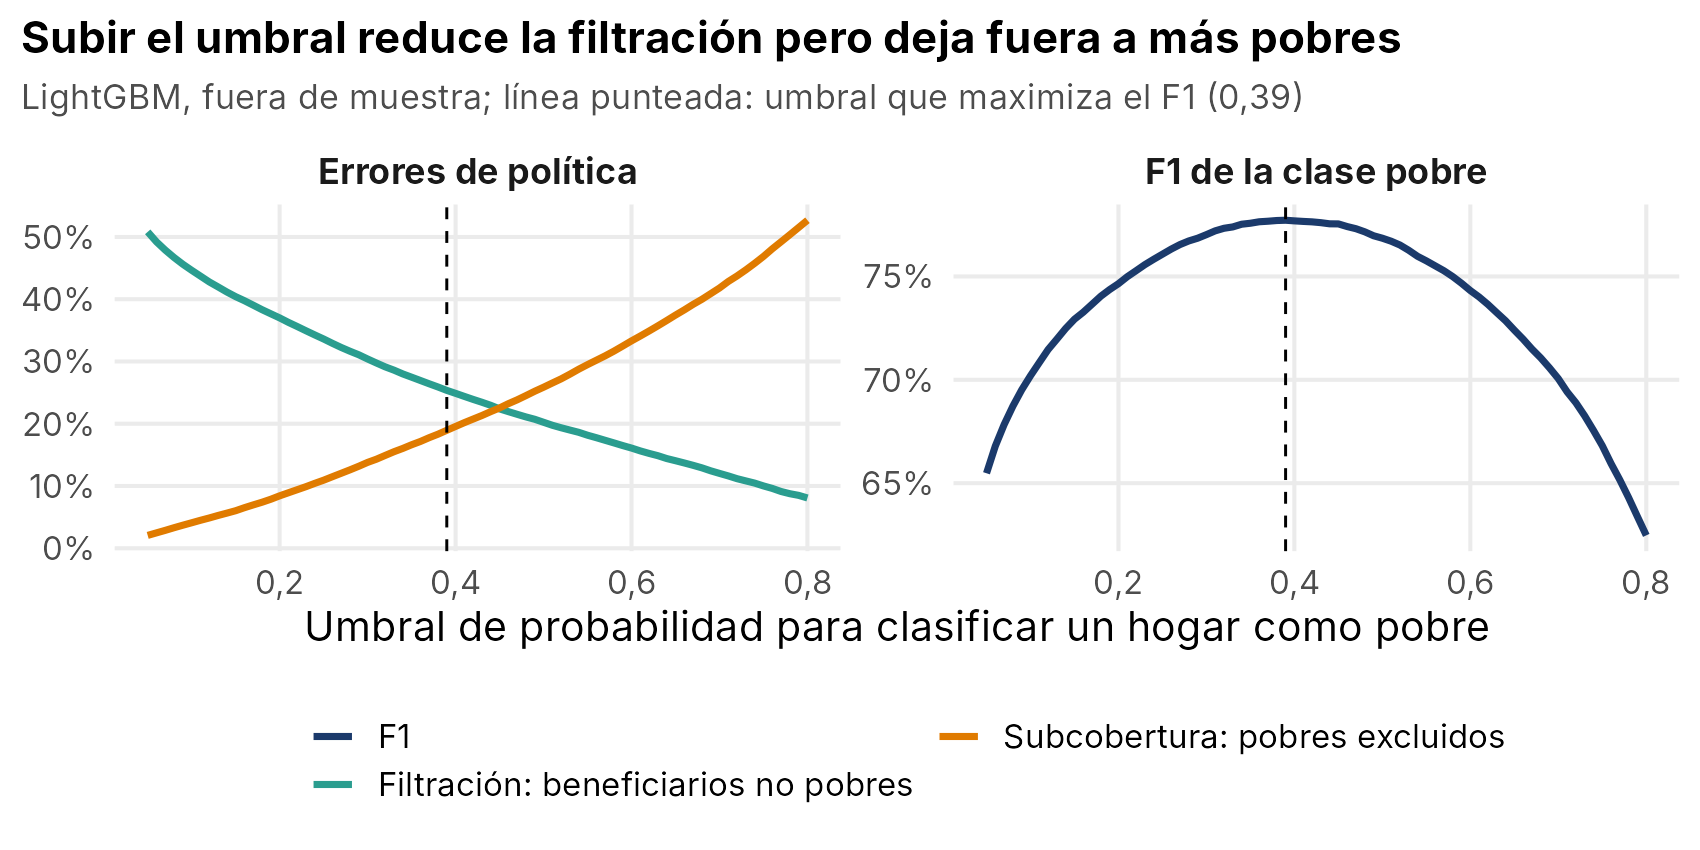
\includegraphics[width=\linewidth,height=.38\textheight,keepaspectratio,trim=0 53 0 0,clip]{harold_slide_threshold_tradeoff.png}\\[-0.5mm]
    {\scriptsize \lineaLeyenda{azul}{F1}\quad \lineaLeyenda{verde}{Filtración: beneficiarios no pobres}\quad \lineaLeyenda{naranja}{Subcobertura: pobres excluidos}}
  \end{columns}
  \vspace{1.5mm}
  \begin{block}{¿Preferiría un gobierno otro balance?}
    \begin{columns}[c]
      \column{.56\textwidth}
      \centering\footnotesize\setlength{\tabcolsep}{5pt}
      \begin{tabular}{lcc}
        \toprule
        \textbf{Umbral} & \textbf{Pobres excluidos} & \textbf{Beneficiarios no pobres}\\
        \midrule
        0,50 & \nUnderAtHalf\,\% & \nLeakAtHalf\,\%\\
        \resaltar{\nThrLGBM{} (máx. F1)} & \resaltar{\nUnderLGBM\,\%} & \resaltar{\nLeakLGBM\,\%}\\
        \nThrUnderTen & 10\,\% & \nLeakAtUnderTen\,\%\\
        \bottomrule
      \end{tabular}\\[0.5mm]
      \fuente{Validación cruzada de 5 pliegues, sin Bogotá.}
      \column{.42\textwidth}
      \footnotesize\raggedright
      Para dejar fuera a solo 10\,\% de los pobres haría falta un umbral de \nThrUnderTen{}, y la filtración subiría a \nLeakAtUnderTen{}\,\%. El costo fiscal de ese equilibrio lo decide la política, no el F1.
    \end{columns}
  \end{block}
\end{frame}

\begin{frame}{Política: los pobres de hogares pequeños son los que más se quedan fuera}
  \begin{columns}[T]
    \column{.66\textwidth}
    \figura{harold_slide_errors_by_group.png}
    \column{.32\textwidth}
    \small
    \begin{itemize}\setlength{\itemsep}{3pt}
      \item La subcobertura casi no cambia entre cabecera (\nUnderCabecera\,\%) y resto rural (\nUnderRestorural\,\%).
      \item Pero es mucho mayor en hogares de 1--2 personas (hipótesis: con pocos perceptores, un error en el ingreso imputado cambia al hogar de lado de la línea).
      \item Un instrumento de focalización debería \resaltar{revisar con visita} a estos hogares en el umbral.
    \end{itemize}
  \end{columns}
\end{frame}

\begin{frame}{Política: la encuesta corta depende de cuántas preguntas exige el ingreso imputado}
  \begin{columns}[T]
    \column{.62\textwidth}
    \figura{harold_slide_short_survey.png}
    \column{.36\textwidth}
    \small
    \begin{itemize}\setlength{\itemsep}{3pt}
      \item Solo con vivienda, composición y educación (\nNVarsSurveyMin{} variables), el F1 es \nFoneSurveyMin{} y se excluye a \nUnderSurveyMin\,\% de los pobres. Agregar empleo y salud lo lleva a \nFoneSurveyShort{}.
      \item Mi ingreso imputado usa unas 60 variables por persona. Otro modelo del equipo, con 8 variables y una primera etapa de ingreso, llegó a 0,77 público y 0,78 privado: \resaltar{se puede acortar} si esa etapa pide pocas preguntas.
    \end{itemize}
    \vspace{1mm}
    \begin{block}{Recomendación}
      \footnotesize
      Cuestionario corto \emph{con} las pocas preguntas de ingreso más informativas, no sin ellas; el modelo sirve para \resaltar{priorizar} hogares a verificar.
    \end{block}
  \end{columns}
\end{frame}

\end{document}
